\documentclass[journal,12pt,twocolumn]{IEEEtran}

\usepackage{setspace}
\usepackage{gensymb}
\singlespacing
\usepackage[cmex10]{amsmath}

\usepackage{amsthm}

\usepackage{mathrsfs}
\usepackage{txfonts}
\usepackage{stfloats}
\usepackage{bm}
\usepackage{cite}
\usepackage{cases}
\usepackage{subfig}

\usepackage{longtable}
\usepackage{multirow}
\usepackage{caption}

\usepackage{enumitem}
\usepackage{mathtools}
\usepackage{steinmetz}
\usepackage{tikz}
\usepackage{circuitikz}
\usepackage{verbatim}
\usepackage{tfrupee}
\usepackage[breaklinks=true]{hyperref}
\usepackage{graphicx}
\usepackage{tkz-euclide}
\usepackage{float}
\usepackage[version=4]{mhchem}

\usetikzlibrary{calc,math}
\usepackage{listings}
    \usepackage{color}                                            %%
    \usepackage{array}                                            %%
    \usepackage{longtable}                                        %%
    \usepackage{calc}                                             %%
    \usepackage{multirow}                                         %%
    \usepackage{hhline}                                           %%
    \usepackage{ifthen}                                           %%
    \usepackage{lscape}     
\usepackage{multicol}
\usepackage{chngcntr}

\DeclareMathOperator*{\Res}{Res}

\renewcommand\thesection{\arabic{section}}
\renewcommand\thesubsection{\thesection.\arabic{subsection}}
\renewcommand\thesubsubsection{\thesubsection.\arabic{subsubsection}}

\renewcommand\thesectiondis{\arabic{section}}
\renewcommand\thesubsectiondis{\thesectiondis.\arabic{subsection}}
\renewcommand\thesubsubsectiondis{\thesubsectiondis.\arabic{subsubsection}}


\hyphenation{op-tical net-works semi-conduc-tor}
\def\inputGnumericTable{}                                 %%

\lstset{
%language=C,
frame=single, 
breaklines=true,
columns=fullflexible
}
\begin{document}

\newcommand{\BEQA}{\begin{eqnarray}}
\newcommand{\EEQA}{\end{eqnarray}}
\newcommand{\define}{\stackrel{\triangle}{=}}
\bibliographystyle{IEEEtran}
\raggedbottom
\setlength{\parindent}{0pt}
\providecommand{\mbf}{\mathbf}
\providecommand{\pr}[1]{\ensuremath{\Pr\left(#1\right)}}
\providecommand{\qfunc}[1]{\ensuremath{Q\left(#1\right)}}
\providecommand{\sbrak}[1]{\ensuremath{{}\left[#1\right]}}
\providecommand{\lsbrak}[1]{\ensuremath{{}\left[#1\right.}}
\providecommand{\rsbrak}[1]{\ensuremath{{}\left.#1\right]}}
\providecommand{\brak}[1]{\ensuremath{\left(#1\right)}}
\providecommand{\lbrak}[1]{\ensuremath{\left(#1\right.}}
\providecommand{\rbrak}[1]{\ensuremath{\left.#1\right)}}
\providecommand{\cbrak}[1]{\ensuremath{\left\{#1\right\}}}
\providecommand{\lcbrak}[1]{\ensuremath{\left\{#1\right.}}
\providecommand{\rcbrak}[1]{\ensuremath{\left.#1\right\}}}
\theoremstyle{remark}
\newtheorem{rem}{Remark}
\newcommand{\sgn}{\mathop{\mathrm{sgn}}}
\providecommand{\abs}[1]{\vert#1\vert}
\providecommand{\res}[1]{\Res\displaylimits_{#1}} 
\providecommand{\norm}[1]{\lVert#1\rVert}
%\providecommand{\norm}[1]{\lVert#1\rVert}
\providecommand{\mtx}[1]{\mathbf{#1}}
\providecommand{\mean}[1]{E[ #1 ]}
\providecommand{\fourier}{\overset{\mathcal{F}}{ \rightleftharpoons}}
%\providecommand{\hilbert}{\overset{\mathcal{H}}{ \rightleftharpoons}}
\providecommand{\system}{\overset{\mathcal{H}}{ \longleftrightarrow}}

	%\newcommand{\solution}[2]{\textbf{Solution:}{#1}}
\newcommand{\solution}{\noindent \textbf{Solution: }}
\newcommand{\cosec}{\,\text{cosec}\,}
\providecommand{\dec}[2]{\ensuremath{\overset{#1}{\underset{#2}{\gtrless}}}}
\newcommand{\myvec}[1]{\ensuremath{\begin{pmatrix}#1\end{pmatrix}}}
\newcommand{\mydet}[1]{\ensuremath{\begin{vmatrix}#1\end{vmatrix}}}
\newcommand\comb[2][^n]{\prescript{#1\mkern-0.5mu}{}C_{#2}}

\numberwithin{equation}{subsection}
\makeatletter
\@addtoreset{figure}{problem}
\makeatother
\let\StandardTheFigure\thefigure
\let\vec\mathbf
\renewcommand{\thefigure}{\theproblem}
\def\putbox#1#2#3{\makebox[0in][l]{\makebox[#1][l]{}\raisebox{\baselineskip}[0in][0in]{\raisebox{#2}[0in][0in]{#3}}}}
     \def\rightbox#1{\makebox[0in][r]{#1}}
     \def\centbox#1{\makebox[0in]{#1}}
     \def\topbox#1{\raisebox{-\baselineskip}[0in][0in]{#1}}
     \def\midbox#1{\raisebox{-0.5\baselineskip}[0in][0in]{#1}}
\vspace{3cm}

\title{AI1103-Assignment-6}
\author{Name: Vikhyath Sai Kothamasu\\Roll Number: CS20BTECH11056}
\maketitle
\newpage
\bigskip
\renewcommand{\thefigure}{\theenumi}
\renewcommand{\thetable}{\theenumi}

\begin{figure} [h]
    \includegraphics[width = 0.8\columnwidth]{college logo.png}
\end{figure}

Download all python codes from 
\begin{lstlisting}
https://github.com/Vikhyath-vec/AI1103/tree/main/Assignment-6/codes
\end{lstlisting}
%
and latex-tikz codes from 
%
\begin{lstlisting}

https://github.com/Vikhyath-vec/AI1103/blob/main/Assignment-6/Assignment-6.tex
\end{lstlisting}
\section*{Question}

Consider an unbiased cubic dice with opposite faces coloured identically and each face coloured red, blue or green such that each colour appears only two times on the dice. If the dice is thrown thrice, the probability of obtaining red colour on top face of the dice at least twice is $\rule{1.6cm}{0.15mm}$ .

\section*{Solution}
Let $X \in \{ 0, 1, 2, 3\}$ be the random variable representing the number of times a red face is obtained. Then $X$ is a binomial distributions with parameter:
\begin{align}
    p &= \frac{\text{number of red coloured faces}}{\text{total number of faces}}
    \\ &= \frac{2}{6}
    \\ &= \frac{1}{3}
\end{align}
Then,
\begin{align}
    \Pr(X=i) = 
	\begin{cases}
	\comb[3]{i}(p)^i(1-p)^{3-i} &  i \in \{0, 1, 2, 3\}\\ ~\\[-1em]
	0 & \text{otherwise}
	\end{cases}
	\\\Pr(X=i) = 
	\begin{cases}
	\comb[3]{i}(\frac{1}{3})^i(1-\frac{1}{3})^{3-i}  &  i \in \{0, 1, 2, 3\}\\ ~\\[-1em]
	0 & \text{otherwise}
	\end{cases}
\end{align}
\begin{center}
\begin{table}[h]
    \centering
    \resizebox{\columnwidth}{!}{
\begin{tabular}{|c|c|c|}
\hline
Serial number & Case & Probability of the case \\
\hline
1 & $\Pr(X=0)$ & $\comb[3]{0}\brak{\frac{1}{3}}^0\brak{\frac{2}{3}}^3 = \frac{8}{27}$ \\ 
\hline
2 & $\Pr(X=1)$ & $\comb[3]{1}\brak{\frac{1}{3}}^1\brak{\frac{2}{3}}^2 = \frac{12}{27}$ \\ 
\hline
3 & $\Pr(X=2)$ & $\comb[3]{2}\brak{\frac{1}{3}}^2\brak{\frac{2}{3}}^1 = \frac{6}{27}$ \\
\hline
4 & $\Pr(X=3)$ & $\comb[3]{3}\brak{\frac{1}{3}}^3\brak{\frac{2}{3}}^0 = \frac{1}{27}$ \\
\hline
\end{tabular}
}
    \caption{PMF of X}
    \label{table 1}
\end{table}
\end{center}
\begin{align}
    F_X(i) = 
	\begin{cases}
	\sum_{k=0}^i\comb[3]{k}(p)^k(1-p)^{3-k} &  i \in \{0, 1, 2, 3\}\\ ~\\[-1em]
	0 & \text{otherwise}
	\end{cases}
\end{align}
\begin{center}
\begin{table}[h]
    \centering
    \resizebox{\columnwidth}{!}{
\begin{tabular}{|c|c|c|}
\hline
Serial number & Case & Cumulative Probability of the case \\
\hline
1 & $F_X(0)$ & $\frac{8}{27}$ \\ 
\hline
2 & $F_X(1)$ & $\frac{8}{27} + \frac{12}{27} = \frac{20}{27}$ \\ 
\hline
3 & $F_X(2)$ & $\frac{8}{27} + \frac{12}{27} + \frac{6}{27} = \frac{26}{27}$ \\
\hline
4 & $F_X(3)$ & $\frac{8}{27} + \frac{12}{27} + \frac{6}{27} + \frac{1}{27} = \frac{27}{27}$ \\
\hline
\end{tabular}
}
    \caption{CDF of X}
    \label{table 2}
\end{table}
\end{center}
\begin{align}
    \Pr{(X \geq 2)} &= 1 - \Pr{(X < 2)}
    \\&= 1 - \Pr{(X \leq 1)}
    \\&= 1 - F_X(1)
    \\&= 1 - \frac{20}{27}
    \\&= \frac{7}{27}
\end{align}
Thus, the probability of obtaining red colour on top face of the dice at least twice is $\frac{7}{27} = 0.25926$.
\begin{figure} [H]
    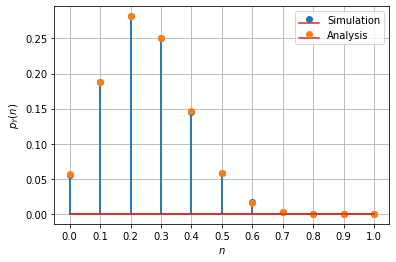
\includegraphics[width = 0.9\columnwidth]{pmf.png}
    \caption{The PMF distribution of $X$}
    \label{Fig 1}
\end{figure}
\begin{figure} [H]
    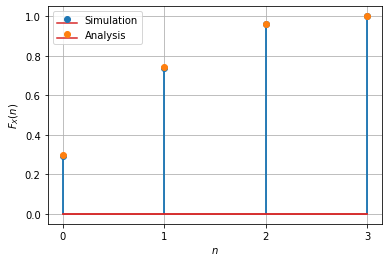
\includegraphics[width = 0.9\columnwidth]{cdf.png}
    \caption{The CDF distribution of $X$}
    \label{Fig 2}
\end{figure}
\end{document}